\chapter{Results} \label{ch:results}


\section{Text Classification}

Quantitative results for Tweet Sentiment Extraction, IMDB, and LIAR are presented in \Cref{tab:tweet}, \Cref{tab:imdb}, and \Cref{tab:politifact}, respectively. Radar plots of the metrics is also reported in \Cref{fig:radar_text}. In all three datasets, our method yields the lowest complexity score and consistently achieves the second-best sparsity score after Saliency. Instead, Guided Backpropagation is the method that performs best in terms of average drop while DeepLIFT has better results in terms of deletion AUC. Also, as an overall behavior across the three datasets, we can observe that Integrated Gradients, DeepLIFT, DeepLIFT-SHAP, Gradient-SHAP, and Guided Backpropagation all result in high complexity and low sparsity. Saliency instead is the worst performing in terms of average drop and deletion AUC, but achieves the best sparsity and reasonable complexity. This highlights a clear trade-off that these methods exhibit between producing attribution maps that are visually appealing and more faithful to the model prediction.

\begin{table}[t!]
    \centering
    \caption{Results for Tweet Sentiment Extraction} \label{tab:tweet}
    \small
    \def\arraystretch{0.75}
    \makebox[\linewidth][c]{%
    \begin{tabular}{lcccc}
        \toprule
        \textbf{Method} & \textbf{Average drop $\downarrow$} & \textbf{Deletion AUC $\downarrow$} & \textbf{Complexity $\downarrow$} & \textbf{Sparsity $\uparrow$} \\
        \midrule
        Saliency         & 1.91 \std{1.76}          & 2.49 \std{1.78}          & 13.11  \std{3.02}          & \textbf{412.95 \std{158.54}} \\
        Guided Backprop. & \textbf{0.09 \std{0.19}} & \textbf{1.38 \std{0.98}} & 312.17 \std{33.18}         & 2.03   \std{0.23} \\
        Int. Gradients   & 0.20 \std{0.57}          & 1.68 \std{1.43}          & 279.29 \std{107.56}        & 2.80   \std{1.90} \\
        DeepLIFT         & 0.42 \std{0.86}          & 1.47 \std{1.25}          & 311.62 \std{101.81}        & 2.31   \std{1.04} \\
        DeepLIFT-SHAP    & 0.44 \std{0.90}          & 1.43 \std{1.19}          & 311.00 \std{87.70}         & 2.22   \std{0.83} \\
        Gradient-SHAP    & 0.34 \std{0.82}          & 1.43 \std{1.22}          & 298.72 \std{99.06}         & 2.40   \std{1.00} \\
        Ours             & 1.11 \std{1.52}          & 1.61 \std{1.57}          & \textbf{2.71   \std{1.04}} & 87.21  \std{72.40} \\
        \bottomrule
    \end{tabular}
    }
\end{table}

\begin{table}[t!]
    \centering
    \caption{Results for IMDB} \label{tab:imdb}
    \small
    \def\arraystretch{0.75}
    \makebox[\linewidth][c]{%
    \begin{tabular}{lcccc}
        \toprule
        \textbf{Method} & \textbf{Average drop $\downarrow$} & \textbf{Deletion AUC $\downarrow$} & \textbf{Complexity $\downarrow$} & \textbf{Sparsity $\uparrow$} \\
        \midrule
        Saliency         & 3.19 \std{1.04}          & 3.06 \std{0.99}          & 18.57  \std{5.97}            & \textbf{114.05 \std{91.08}} \\
        Guided Backprop. & \textbf{0.05 \std{0.14}} & 1.62 \std{0.56}          & 313.09 \std{41.16}           & 2.04   \std{0.29} \\
        Int. Gradients   & 0.72 \std{1.39}          & 1.76 \std{1.06}          & 279.72 \std{171.69}          & 4.37   \std{4.96} \\
        DeepLIFT         & 0.15 \std{0.63}          & 1.61 \std{0.81}          & 315.50 \std{108.50}          & 2.35   \std{1.23} \\
        DeepLIFT-SHAP    & 0.14 \std{0.63}          & \textbf{1.58 \std{0.78}} & 315.62 \std{103.78}          & 2.32   \std{1.20} \\
        Gradient-SHAP    & 0.10 \std{0.50}          & 1.66 \std{0.81}          & 296.16 \std{111.63}          & 2.52   \std{1.24} \\
        Ours             & 0.46 \std{0.63}          & 1.83 \std{0.76}          & \textbf{4.90   \std{2.22}}   & 12.64  \std{12.29} \\
        \bottomrule
    \end{tabular}
    }
\end{table}

\begin{table}[t!]
    \centering
    \caption{Results for LIAR} \label{tab:politifact}
    \small
    \def\arraystretch{0.75}
    \makebox[\linewidth][c]{%
    \begin{tabular}{lcccc}
        \toprule
        \textbf{Method} & \textbf{Average drop $\downarrow$} & \textbf{Deletion AUC $\downarrow$} & \textbf{Complexity $\downarrow$} & \textbf{Sparsity $\uparrow$} \\
        \midrule
        Saliency         & 1.44 \std{1.20}          & 1.36 \std{1.14}          & 16.59  \std{5.93}            & \textbf{104.42 \std{85.75}} \\
        Guided Backprop. & \textbf{0.09 \std{0.16}} & 0.74 \std{0.61}          & 316.11 \std{46.54}           & 2.03   \std{0.32} \\
        Int. Gradients   & 0.23 \std{0.61}          & 0.85 \std{0.81}          & 278.28 \std{109.90}          & 2.75   \std{1.50} \\
        DeepLIFT         & 0.21 \std{0.52}          & \textbf{0.72 \std{0.68}} & 323.70 \std{123.19}          & 2.36   \std{1.26} \\
        DeepLIFT-SHAP    & 0.20 \std{0.54}          & 0.73 \std{0.68}          & 323.81 \std{116.52}          & 2.31   \std{1.23} \\
        Gradient-SHAP    & 0.17 \std{0.49}          & 0.73 \std{0.68}          & 312.24 \std{119.44}          & 2.52   \std{1.73} \\
        Ours             & 0.26 \std{0.29}          & 1.00 \std{0.80}          & \textbf{7.71   \std{0.34}}   & 3.08   \std{1.63} \\
        \bottomrule
    \end{tabular}
    }
\end{table}

\begin{figure}[t!]
    \centering
    \begin{subfigure}[c]{0.26\linewidth}
        \centering
        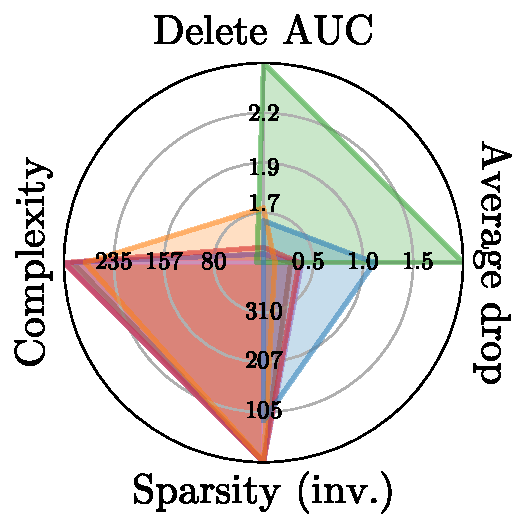
\includegraphics[scale=0.4]{./img/radar-tweet.pdf}
        \caption{Tweet Sentiment}
    \end{subfigure}
    \begin{subfigure}[c]{0.26\linewidth}
        \centering
        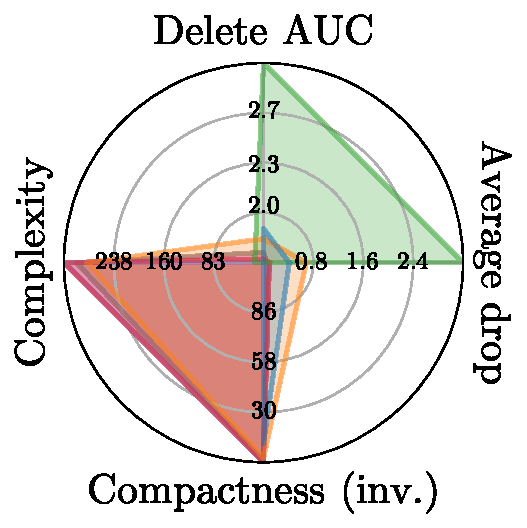
\includegraphics[scale=0.4]{./img/radar-imdb.pdf}
        \caption{IMDB}
    \end{subfigure}
    \begin{subfigure}[c]{0.26\linewidth}
        \centering
        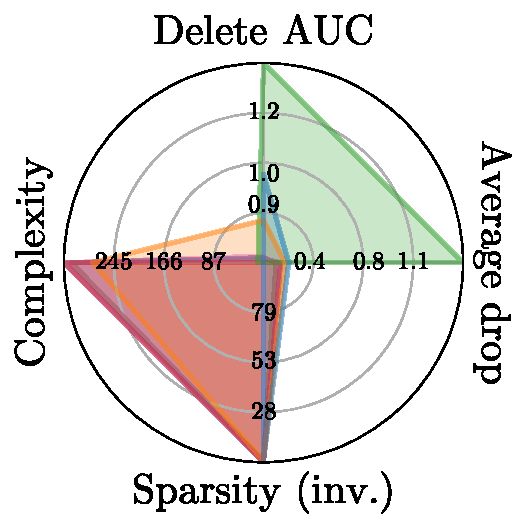
\includegraphics[scale=0.4]{./img/radar-politifact.pdf}
        \caption{LIAR}
    \end{subfigure}
    \begin{subfigure}[c]{0.16\linewidth}
        \centering
        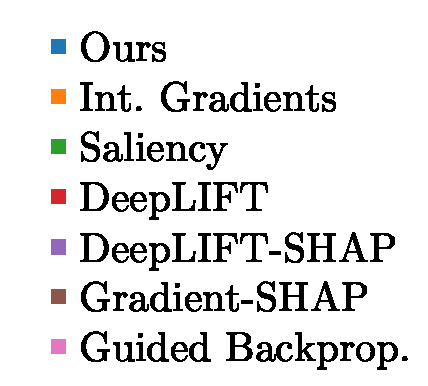
\includegraphics[scale=0.4]{./img/radar-legend.pdf}
    \end{subfigure}
    \caption{Radar plot of the quantitative metrics for the text tasks. The closer to the center, the better.} \label{fig:radar_text}
\end{figure}

Qualitatively, we manually evaluate some samples from IMDB. We choose this dataset as it has longer documents compared to Tweet Sentiment Extraction and its classifier achieves near perfect results, which should make it easier to intuitively evaluate the attribution maps. We selected 100 random samples from the dataset and evaluated them. The main pattern we observed is that our method, compared to the other baselines, has a more decisive scoring system as it favors either very high or very low scores, while the other methods tend to give some degree of importance to each token. Also, we observed that the attribution scores correctly highlight the most relevant terms to decide the sentiment, although it frequently also highlights surrounding terms which are not necessarily relevant according to human intuition. We report in \Cref{fig:imdb_sample} a sample extracted from the dataset. Moreover, in line with the metrics, Integrated Gradients, DeepLIFT, DeepLIFT-SHAP, Gradient-SHAP, and Guided Backpropagation are the methods that produce attribution maps that span across the whole input the most, while Saliency is the method where the scores are more concentrated on a few words.

\begin{figure}[t!]
    \scriptsize
    \centering
    \makebox[\linewidth][c]{%
    \begin{tabular}{lc}
    \textbf{Ours} & {\tt\colorbox[RGB]{221, 62, 42}{\textcolor{black}{\vphantom{Tg}This}} \colorbox[RGB]{249, 132, 85}{\textcolor{black}{\vphantom{Tg}is}} \colorbox[RGB]{217, 52, 34}{\textcolor{black}{\vphantom{Tg}a}} \colorbox[RGB]{190, 15, 10}{\textcolor{white}{\vphantom{Tg}great}} \colorbox[RGB]{207, 38, 24}{\textcolor{white}{\vphantom{Tg}movie.}} \colorbox[RGB]{253, 220, 175}{\textcolor{black}{\vphantom{Tg}Too}} \colorbox[RGB]{255, 243, 226}{\textcolor{black}{\vphantom{Tg}bad}} \colorbox[RGB]{253, 168, 114}{\textcolor{black}{\vphantom{Tg}it}} \colorbox[RGB]{253, 171, 117}{\textcolor{black}{\vphantom{Tg}is}} \colorbox[RGB]{254, 224, 183}{\textcolor{black}{\vphantom{Tg}not}} \colorbox[RGB]{255, 244, 228}{\textcolor{black}{\vphantom{Tg}available}} \colorbox[RGB]{255, 247, 235}{\textcolor{black}{\vphantom{Tg}on}} \colorbox[RGB]{255, 243, 227}{\textcolor{black}{\vphantom{Tg}home}} \colorbox[RGB]{252, 149, 96}{\textcolor{black}{\vphantom{Tg}video.</s>}}}\\
    \textbf{Saliency} & {\tt\colorbox[RGB]{253, 171, 117}{\textcolor{black}{\vphantom{Tg}This}} \colorbox[RGB]{253, 199, 145}{\textcolor{black}{\vphantom{Tg}is}} \colorbox[RGB]{253, 190, 135}{\textcolor{black}{\vphantom{Tg}a}} \colorbox[RGB]{127, 0, 0}{\textcolor{white}{\vphantom{Tg}great}} \colorbox[RGB]{236, 95, 67}{\textcolor{black}{\vphantom{Tg}movie.}} \colorbox[RGB]{253, 197, 142}{\textcolor{black}{\vphantom{Tg}Too}} \colorbox[RGB]{253, 191, 137}{\textcolor{black}{\vphantom{Tg}bad}} \colorbox[RGB]{253, 208, 154}{\textcolor{black}{\vphantom{Tg}it}} \colorbox[RGB]{253, 221, 177}{\textcolor{black}{\vphantom{Tg}is}} \colorbox[RGB]{253, 216, 167}{\textcolor{black}{\vphantom{Tg}not}} \colorbox[RGB]{253, 165, 111}{\textcolor{black}{\vphantom{Tg}available}} \colorbox[RGB]{253, 216, 167}{\textcolor{black}{\vphantom{Tg}on}} \colorbox[RGB]{252, 160, 107}{\textcolor{black}{\vphantom{Tg}home}} \colorbox[RGB]{253, 181, 126}{\textcolor{black}{\vphantom{Tg}video.</s>}}}\\
    \textbf{Guided backprop} & {\tt\colorbox[RGB]{252, 152, 99}{\textcolor{black}{\vphantom{Tg}This}} \colorbox[RGB]{227, 75, 52}{\textcolor{black}{\vphantom{Tg}is}} \colorbox[RGB]{188, 12, 8}{\textcolor{white}{\vphantom{Tg}a}} \colorbox[RGB]{253, 186, 131}{\textcolor{black}{\vphantom{Tg}great}} \colorbox[RGB]{253, 213, 160}{\textcolor{black}{\vphantom{Tg}movie.}} \colorbox[RGB]{253, 199, 145}{\textcolor{black}{\vphantom{Tg}Too}} \colorbox[RGB]{239, 101, 72}{\textcolor{black}{\vphantom{Tg}bad}} \colorbox[RGB]{252, 163, 110}{\textcolor{black}{\vphantom{Tg}it}} \colorbox[RGB]{202, 30, 20}{\textcolor{white}{\vphantom{Tg}is}} \colorbox[RGB]{215, 48, 31}{\textcolor{black}{\vphantom{Tg}not}} \colorbox[RGB]{179, 0, 0}{\textcolor{white}{\vphantom{Tg}available}} \colorbox[RGB]{244, 117, 79}{\textcolor{black}{\vphantom{Tg}on}} \colorbox[RGB]{127, 0, 0}{\textcolor{white}{\vphantom{Tg}home}} \colorbox[RGB]{253, 175, 121}{\textcolor{black}{\vphantom{Tg}video.</s>}}}\\
    \textbf{Int. Gradients} & {\tt\colorbox[RGB]{142, 0, 0}{\textcolor{white}{\vphantom{Tg}This}} \colorbox[RGB]{250, 134, 86}{\textcolor{black}{\vphantom{Tg}is}} \colorbox[RGB]{249, 130, 84}{\textcolor{black}{\vphantom{Tg}a}} \colorbox[RGB]{127, 0, 0}{\textcolor{white}{\vphantom{Tg}great}} \colorbox[RGB]{229, 80, 56}{\textcolor{black}{\vphantom{Tg}movie.}} \colorbox[RGB]{226, 72, 49}{\textcolor{black}{\vphantom{Tg}Too}} \colorbox[RGB]{248, 129, 84}{\textcolor{black}{\vphantom{Tg}bad}} \colorbox[RGB]{251, 139, 88}{\textcolor{black}{\vphantom{Tg}it}} \colorbox[RGB]{253, 175, 121}{\textcolor{black}{\vphantom{Tg}is}} \colorbox[RGB]{255, 247, 236}{\textcolor{black}{\vphantom{Tg}not}} \colorbox[RGB]{253, 171, 117}{\textcolor{black}{\vphantom{Tg}available}} \colorbox[RGB]{252, 149, 96}{\textcolor{black}{\vphantom{Tg}on}} \colorbox[RGB]{232, 85, 60}{\textcolor{black}{\vphantom{Tg}home}} \colorbox[RGB]{244, 118, 79}{\textcolor{black}{\vphantom{Tg}video.</s>}}}\\
    \textbf{DeepLIFT} & {\tt\colorbox[RGB]{249, 130, 84}{\textcolor{black}{\vphantom{Tg}This}} \colorbox[RGB]{239, 101, 72}{\textcolor{black}{\vphantom{Tg}is}} \colorbox[RGB]{237, 97, 69}{\textcolor{black}{\vphantom{Tg}a}} \colorbox[RGB]{253, 194, 139}{\textcolor{black}{\vphantom{Tg}great}} \colorbox[RGB]{252, 140, 89}{\textcolor{black}{\vphantom{Tg}movie.}} \colorbox[RGB]{253, 165, 111}{\textcolor{black}{\vphantom{Tg}Too}} \colorbox[RGB]{240, 105, 74}{\textcolor{black}{\vphantom{Tg}bad}} \colorbox[RGB]{246, 123, 81}{\textcolor{black}{\vphantom{Tg}it}} \colorbox[RGB]{251, 137, 87}{\textcolor{black}{\vphantom{Tg}is}} \colorbox[RGB]{252, 147, 95}{\textcolor{black}{\vphantom{Tg}not}} \colorbox[RGB]{218, 55, 36}{\textcolor{black}{\vphantom{Tg}available}} \colorbox[RGB]{242, 109, 75}{\textcolor{black}{\vphantom{Tg}on}} \colorbox[RGB]{234, 90, 63}{\textcolor{black}{\vphantom{Tg}home}} \colorbox[RGB]{243, 113, 77}{\textcolor{black}{\vphantom{Tg}video.</s>}}}\\
    \textbf{DeepLIFT-SHAP} & {\tt\colorbox[RGB]{248, 129, 84}{\textcolor{black}{\vphantom{Tg}This}} \colorbox[RGB]{242, 109, 75}{\textcolor{black}{\vphantom{Tg}is}} \colorbox[RGB]{241, 108, 75}{\textcolor{black}{\vphantom{Tg}a}} \colorbox[RGB]{253, 194, 139}{\textcolor{black}{\vphantom{Tg}great}} \colorbox[RGB]{252, 140, 89}{\textcolor{black}{\vphantom{Tg}movie.}} \colorbox[RGB]{252, 160, 107}{\textcolor{black}{\vphantom{Tg}Too}} \colorbox[RGB]{230, 82, 57}{\textcolor{black}{\vphantom{Tg}bad}} \colorbox[RGB]{241, 106, 74}{\textcolor{black}{\vphantom{Tg}it}} \colorbox[RGB]{249, 133, 86}{\textcolor{black}{\vphantom{Tg}is}} \colorbox[RGB]{249, 133, 86}{\textcolor{black}{\vphantom{Tg}not}} \colorbox[RGB]{205, 35, 22}{\textcolor{white}{\vphantom{Tg}available}} \colorbox[RGB]{242, 110, 76}{\textcolor{black}{\vphantom{Tg}on}} \colorbox[RGB]{236, 95, 67}{\textcolor{black}{\vphantom{Tg}home}} \colorbox[RGB]{243, 113, 77}{\textcolor{black}{\vphantom{Tg}video.</s>}}}\\
    \textbf{Gradient-SHAP} & {\tt\colorbox[RGB]{251, 139, 88}{\textcolor{black}{\vphantom{Tg}This}} \colorbox[RGB]{254, 232, 200}{\textcolor{black}{\vphantom{Tg}is}} \colorbox[RGB]{253, 187, 133}{\textcolor{black}{\vphantom{Tg}a}} \colorbox[RGB]{127, 0, 0}{\textcolor{white}{\vphantom{Tg}great}} \colorbox[RGB]{217, 52, 34}{\textcolor{black}{\vphantom{Tg}movie.}} \colorbox[RGB]{248, 129, 84}{\textcolor{black}{\vphantom{Tg}Too}} \colorbox[RGB]{255, 247, 236}{\textcolor{black}{\vphantom{Tg}bad}} \colorbox[RGB]{253, 173, 119}{\textcolor{black}{\vphantom{Tg}it}} \colorbox[RGB]{253, 200, 146}{\textcolor{black}{\vphantom{Tg}is}} \colorbox[RGB]{253, 216, 167}{\textcolor{black}{\vphantom{Tg}not}} \colorbox[RGB]{244, 117, 79}{\textcolor{black}{\vphantom{Tg}available}} \colorbox[RGB]{245, 119, 80}{\textcolor{black}{\vphantom{Tg}on}} \colorbox[RGB]{244, 118, 79}{\textcolor{black}{\vphantom{Tg}home}} \colorbox[RGB]{253, 217, 170}{\textcolor{black}{\vphantom{Tg}video.</s>}}}\\
    \end{tabular}
    }
    \caption{Sample from IMDB} \label{fig:imdb_sample}
\end{figure}

Putting all these observations together, we can conclude that our method, being the one with the least complexity metric and with generally higher sparsity, produces attribution maps that are closer to binary masks, indicating that it gives a clear distinction between what the classifier is considering relevant and what it is not, making its attribution maps generally more appealing. Moreover, by achieving decent average drop and deletion AUC, it shows that it is able to highlight relevant features of the input space, which indicates that it does not lose in faithfulness.



\section{Image Classification}
For the image classification tasks, we report the result for MNIST, CIFAR-10, and Imagenette on \Cref{tab:mnist}, \Cref{tab:cifar10}, and \Cref{tab:imagenette}, respectively, while the radar plots are depicted in \Cref{fig:radar_image}. For these datasets, our method consistently achieves the highest average drop and deletion AUC. In terms of complexity, Integrated Gradients is the method performing the best, while, for sparsity, Saliency has the highest results. Instead, as for the case of text, DeepLIFT, DeepLIFT-SHAP, Gradient-SHAP, and Guided Backpropagation all produce highly complex and weakly compact maps, but achieve high results in terms of average drop and deletion AUC. This highlights again a trade-off between faithfulness and appeal that is present among these methods, and ours is again located as a balanced approach for these two requirements.

\begin{table}[t!]
    \centering
    \caption{Results on MNIST} \label{tab:mnist}
    \small
    \def\arraystretch{0.75}
    \makebox[\linewidth][c]{%
    \begin{tabular}{lcccc}
        \toprule
        \textbf{Method} & \textbf{Average drop $\downarrow$} & \textbf{Deletion AUC $\downarrow$} & \textbf{Complexity $\downarrow$} & \textbf{Sparsity $\uparrow$} \\
        \midrule
        Saliency         & 0.63 \std{0.31}          & 0.81 \std{0.14}          & 13.39  \std{4.57}           & \textbf{42.85 \std{36.35}} \\
        Guided Backprop. & 0.07 \std{0.19}          & 0.45 \std{0.10}          & 112.17 \std{13.22}          & 2.03  \std{0.26} \\
        Int. Gradients   & 0.02 \std{0.09}          & 0.57 \std{0.15}          & \textbf{4.86   \std{1.43}}  & 3.64  \std{1.92} \\
        DeepLIFT         & 0.03 \std{0.13}          & 0.45 \std{0.10}          & 111.46 \std{13.58}          & 2.05  \std{0.27} \\
        DeepLIFT-SHAP    & \textbf{0.01 \std{0.10}} & \textbf{0.44 \std{0.11}} & 111.85 \std{16.12}          & 2.05  \std{0.32} \\
        Gradient-SHAP    & 0.01 \std{0.09}          & \textbf{0.44 \std{0.09}} & 110.89 \std{14.69}          & 2.06  \std{0.29} \\
        Ours              & \textbf{0.01 \std{0.08}} & 0.53 \std{0.26}          & 33.65  \std{15.36}          & 22.20 \std{10.97} \\
        \bottomrule
    \end{tabular}
    }
\end{table}

\begin{table}[t!]
    \centering
    \caption{Results on CIFAR-10} \label{tab:cifar10}
    \small
    \def\arraystretch{0.75}
    \makebox[\linewidth][c]{%
    \begin{tabular}{lcccc}
        \toprule
        \textbf{Method} & \textbf{Average drop $\downarrow$} & \textbf{Deletion AUC $\downarrow$} & \textbf{Complexity $\downarrow$} & \textbf{Sparsity $\uparrow$} \\
        \midrule
        Saliency         & 0.88 \std{0.09}          & 0.83 \std{0.05}          & 12.49  \std{7.20}           & \textbf{63.91 \std{58.92}} \\
        Guided Backprop. & 0.21 \std{0.37}          & 0.48 \std{0.08}          & 111.92 \std{12.76}          & 2.03  \std{0.24} \\
        Int. Gradients   & \textbf{0.03 \std{0.16}} & 0.57 \std{0.13}          & \textbf{5.75   \std{1.57}}  & 2.84  \std{1.01} \\
        DeepLIFT         & 0.07 \std{0.22}          & \textbf{0.46 \std{0.09}} & 112.75 \std{16.48}          & 2.04  \std{0.32} \\
        DeepLIFT-SHAP    & 0.06 \std{0.21}          & \textbf{0.46 \std{0.09}} & 113.32 \std{16.49}          & 2.02  \std{0.31} \\
        Gradient-SHAP    & 0.05 \std{0.20}          & 0.48 \std{0.08}          & 111.75 \std{13.80}          & 2.04  \std{0.26} \\
        Ours              & \textbf{0.03 \std{0.15}} & 0.52 \std{0.18}          & 68.44  \std{18.32}          & 5.02  \std{2.01} \\
        \bottomrule
    \end{tabular}
    }
\end{table}

\begin{table}[t!]
    \centering
    \caption{Results on Imagenette} \label{tab:imagenette}
    \small
    \def\arraystretch{0.75}
    \makebox[\linewidth][c]{%
    \begin{tabular}{lcccc}
        \toprule
        \textbf{Method} & \textbf{Average drop $\downarrow$} & \textbf{Deletion AUC $\downarrow$} & \textbf{Complexity $\downarrow$} & \textbf{Sparsity $\uparrow$} \\
        \midrule
        Saliency         & 0.50 \std{0.17}          & 0.53 \std{0.09}          & 10.46  \std{5.07}           & \textbf{73.55 \std{60.17}} \\
        Guided Backprop. & 0.05 \std{0.11}          & 0.28 \std{0.06}          & 112.95 \std{12.52}          & 2.01  \std{0.23} \\
        Int. Gradients   & \textbf{0.01 \std{0.06}} & 0.31 \std{0.11}          & \textbf{5.79   \std{1.76}}  & 2.87  \std{1.20} \\
        DeepLIFT         & \textbf{0.01 \std{0.07}} & 0.28 \std{0.06}          & 112.46 \std{15.83}          & 2.04  \std{0.32} \\
        DeepLIFT-SHAP    & \textbf{0.01 \std{0.07}} & 0.28 \std{0.06}          & 112.46 \std{16.02}          & 2.04  \std{0.31} \\
        Gradient-SHAP    & \textbf{0.01 \std{0.06}} & 0.28 \std{0.06}          & 110.71 \std{14.36}          & 2.06  \std{0.29} \\
        Ours              & 0.02 \std{0.07}          & \textbf{0.27 \std{0.12}} & 60.43  \std{19.45}          & 7.02  \std{2.92} \\
        \bottomrule
    \end{tabular}
    }
\end{table}

\begin{figure}[t!]
    \centering
    \begin{subfigure}[c]{0.26\linewidth}
        \centering
        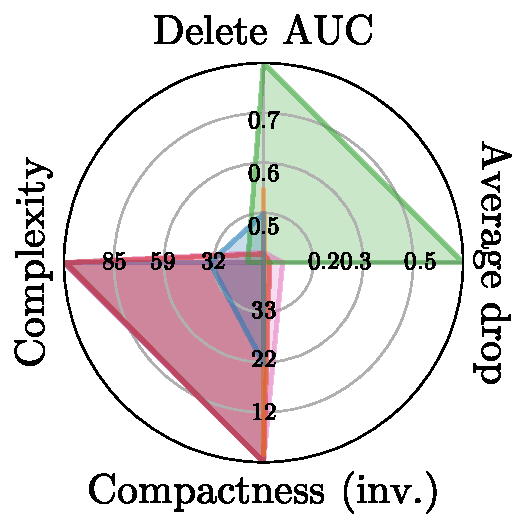
\includegraphics[scale=0.4]{./img/radar-mnist.pdf}
        \caption{MNIST}
    \end{subfigure}
    \begin{subfigure}[c]{0.26\linewidth}
        \centering
        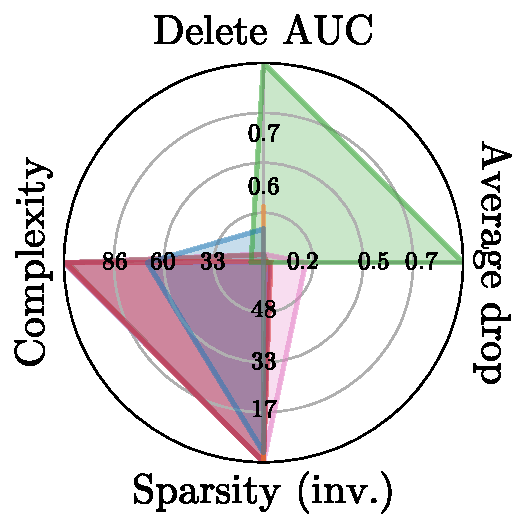
\includegraphics[scale=0.4]{./img/radar-cifar10.pdf}
        \caption{CIFAR-10}
    \end{subfigure}
    \begin{subfigure}[c]{0.26\linewidth}
        \centering
        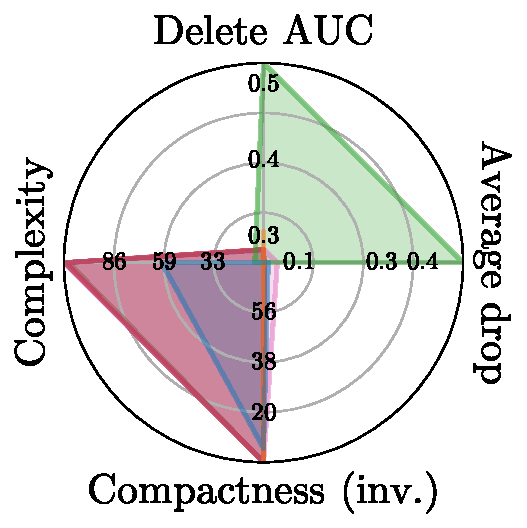
\includegraphics[scale=0.4]{./img/radar-imagenette.pdf}
        \caption{Imagenette}
    \end{subfigure}
    \begin{subfigure}[c]{0.16\linewidth}
        \centering
        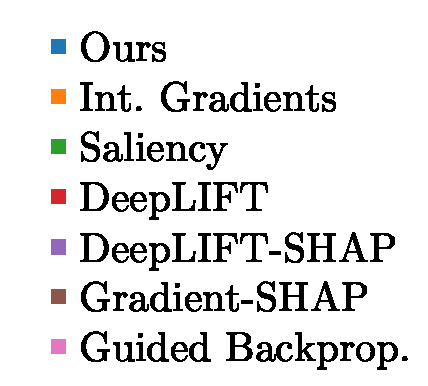
\includegraphics[scale=0.4]{./img/radar-legend.pdf}
    \end{subfigure}
    \caption{Radar plot of the quantitative metrics for the image tasks. The closer to the center, the better.} \label{fig:radar_image}
\end{figure}

Qualitatively, we evaluate 100 random samples from Imagenette. In the case of images, all classifiers have strong performance, therefore, we choose to analyze Imagenette as it contains images of higher resolution. Similarly to the results we obtained for text, we can observe that compared to the other baselines, except Saliency, the attribution map produced with our method is closer to a binary mask with values closer to either $0$ or $1$. Also, compared to gradient-based methods, in the case of images, we can observe that almost all, but Integrated Gradients, produce results that are very focused on a small subset of pixels, which makes results less visually appealing, although performing well in terms of average drop and deletion AUC. Finally, semantically, we observed that almost all attribution maps correctly identify the object of interest in the image by either highlighting it wholly or by identifying key characteristics. We report a sample from the dataset in \Cref{fig:imagenette_sample}.

\begin{figure}[t!]
    \centering
    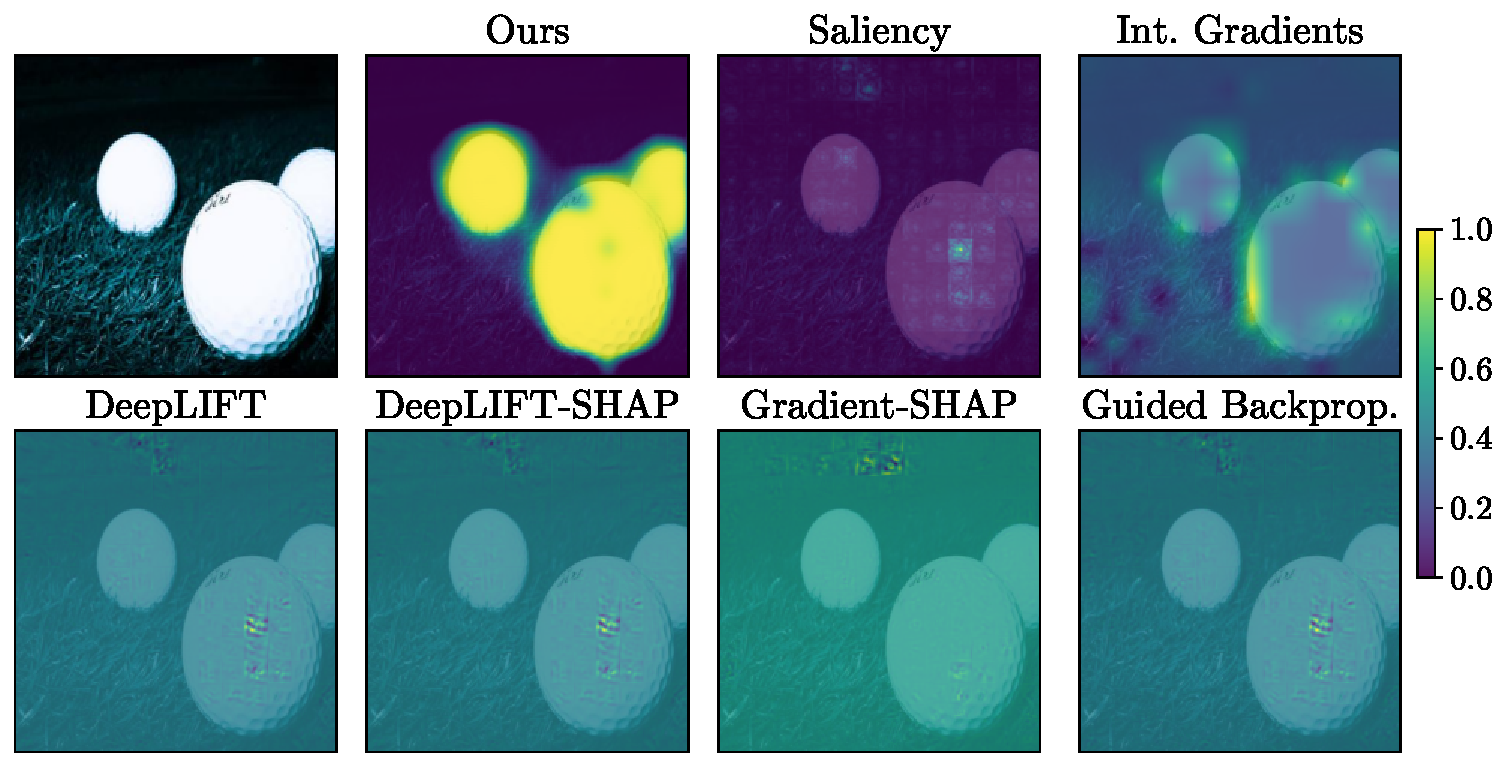
\includegraphics[width=0.9\linewidth]{./img/imagenette.pdf}
    \caption{Sample from Imagenette} \label{fig:imagenette_sample}
\end{figure}

Overall, results with images highlight that, as for text, the attribution maps produced by our method have a clear separation between what is relevant and what is not while also achieving competitive values of average drop and deletion AUC. This again highlights a trade-off between attribution map faithfulness and visual plausibility, and our method is located in the middle ground between the two requirements.



\section{Multimodal Classification}

Results on multimodal datasets are reported in \Cref{tab:flickr8k}, \Cref{tab:hateful_memes}, and \Cref{tab:snli_ve} for Flickr8k, Hateful Memes, and SNLI-VE, respectively, and the radar plots are in \Cref{fig:radar_mm}. Consistent with the previous results, Saliency is the method that achieves the best complexity and sparsity, while the other gradient-based methods perform best in terms of average drop and deletion AUC. Our method again performs with a trade-off between the two sides by achieving competitive average drop while maintaining a lower complexity and higher sparsity.

\begin{table}[t!]
    \centering
    \caption{Results on Flickr8k} \label{tab:flickr8k}
    \small
    \def\arraystretch{0.75}
    \makebox[\linewidth][c]{%
    \begin{tabular}{lcccc}
        \toprule
        \textbf{Method} & \textbf{Average drop $\downarrow$} & \textbf{Deletion AUC $\downarrow$} & \textbf{Complexity $\downarrow$} & \textbf{Sparsity $\uparrow$} \\
        \midrule
        Saliency         & 1.86 \std{1.70}          & 1.79 \std{1.07}          & \textbf{15.20  \std{3.50}}  & \textbf{79.10 \std{36.06}} \\
        Guided Backprop. & \textbf{0.71 \std{0.98}} & \textbf{1.11 \std{0.66}} & 174.10 \std{15.05}          & 2.05 \std{0.18} \\
        Int. Gradients   & 0.77 \std{1.39}          & 1.88 \std{1.15}          & 66.06  \std{30.85}          & 2.82 \std{1.24} \\
        DeepLIFT         & 0.95 \std{1.40}          & 1.32 \std{0.84}          & 180.31 \std{28.94}          & 2.07 \std{0.41} \\
        DeepLIFT-SHAP    & 0.93 \std{1.39}          & 1.20 \std{0.75}          & 174.90 \std{21.89}          & 2.08 \std{0.28} \\
        Gradient-SHAP    & 1.04 \std{1.57}          & 1.24 \std{0.80}          & 177.29 \std{24.94}          & 2.07 \std{0.36} \\
        Ours              & 1.21 \std{1.22}          & 2.04 \std{1.21}          & 38.47  \std{8.74}           & 10.54 \std{2.27} \\
        \bottomrule
    \end{tabular}
    }
\end{table}

\begin{table}[t!]
    \centering
    \caption{Results on Hateful Memes} \label{tab:hateful_memes}
    \small
    \def\arraystretch{0.75}
    \makebox[\linewidth][c]{%
    \begin{tabular}{lcccc}
        \toprule
        \textbf{Method} & \textbf{Average drop $\downarrow$} & \textbf{Deletion AUC $\downarrow$} & \textbf{Complexity $\downarrow$} & \textbf{Sparsity $\uparrow$} \\
        \midrule
        Saliency         & 1.26 \std{1.34}          & 1.25 \std{0.98}          & \textbf{14.80  \std{3.79}}  & \textbf{84.04 \std{36.24}} \\
        Guided Backprop. & 0.92 \std{1.00}          & 0.80 \std{0.53}          & 175.90 \std{14.93}          & 2.03 \std{0.18} \\
        Int. Gradients   & \textbf{0.45 \std{0.98}} & \textbf{0.78 \std{0.58}} & 80.76  \std{22.80}          & 2.28 \std{0.81} \\
        DeepLIFT         & 0.49 \std{0.98}          & 0.81 \std{0.56}          & 172.86 \std{28.59}          & 2.22 \std{0.68} \\
        DeepLIFT-SHAP    & 0.48 \std{0.95}          & 0.82 \std{0.60}          & 168.37 \std{27.26}          & 2.27 \std{0.62} \\
        Gradient-SHAP    & 0.49 \std{0.94}          & \textbf{0.78 \std{0.55}} & 176.54 \std{29.93}          & 2.15 \std{0.57} \\
        Ours              & 0.98 \std{0.99}          & 1.13 \std{0.91}          & 67.60  \std{19.82}          & 15.24 \std{7.94} \\
        \bottomrule
    \end{tabular}
    }
\end{table}

\begin{table}[t!]
    \centering
    \caption{Results on SNLI-VE} \label{tab:snli_ve}
    \small
    \def\arraystretch{0.75}
    \makebox[\linewidth][c]{%
    \begin{tabular}{lcccc}
        \toprule
        \textbf{Method} & \textbf{Average drop $\downarrow$} & \textbf{Deletion AUC $\downarrow$} & \textbf{Complexity $\downarrow$} & \textbf{Sparsity $\uparrow$} \\
        \midrule
        Saliency         & 4.27 \std{1.83}          & 3.89 \std{1.65}          & \textbf{14.41  \std{3.84}}  & \textbf{76.98 \std{35.92}} \\
        Guided Backprop. & 0.27 \std{0.32}          & 2.10 \std{0.86}          & 173.94 \std{14.78}          & 2.05 \std{0.17} \\
        Int. Gradients   & 1.20 \std{2.19}          & 3.19 \std{1.73}          & 48.72  \std{23.55}          & 3.44 \std{1.72} \\
        DeepLIFT         & \textbf{0.06 \std{0.21}} & 2.11 \std{1.05}          & 174.88 \std{22.61}          & 2.09 \std{0.32} \\
        DeepLIFT-SHAP    & \textbf{0.06 \std{0.20}} & 2.11 \std{0.93}          & 173.94 \std{20.18}          & 2.08 \std{0.28} \\
        Gradient-SHAP    & 0.12 \std{0.46}          & \textbf{2.04 \std{0.93}} & 174.89 \std{26.29}          & 2.15 \std{0.50} \\
        Ours              & 0.92 \std{0.83}          & 3.18 \std{1.51}          & 41.68  \std{9.64}           & 11.07 \std{3.80} \\
        \bottomrule
    \end{tabular}
    }
\end{table}

\begin{figure}[t!]
    \centering
    \begin{subfigure}[c]{0.26\linewidth}
        \centering
        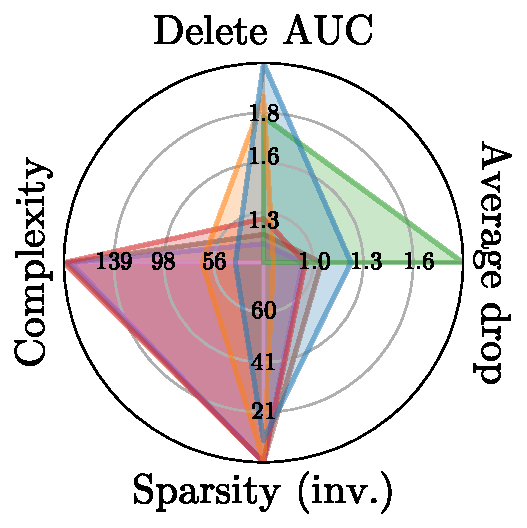
\includegraphics[scale=0.4]{./img/radar-flickr8k.pdf}
        \caption{Flickr8k}
    \end{subfigure}
    \begin{subfigure}[c]{0.26\linewidth}
        \centering
        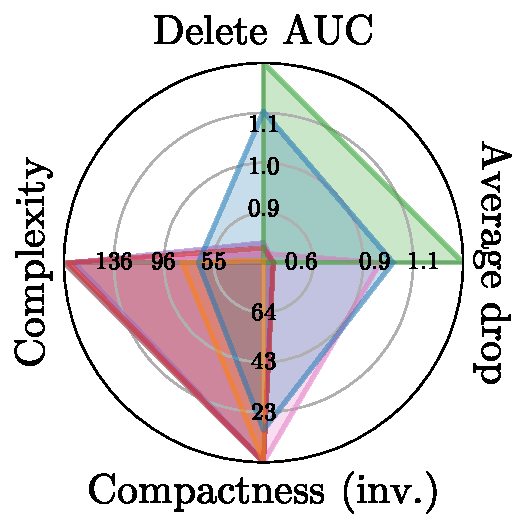
\includegraphics[scale=0.4]{./img/radar-hateful_memes.pdf}
        \caption{Hateful Memes}
    \end{subfigure}
    \begin{subfigure}[c]{0.26\linewidth}
        \centering
        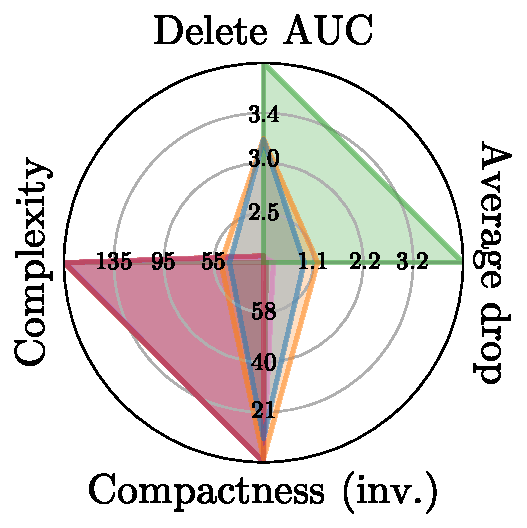
\includegraphics[scale=0.4]{./img/radar-snli_ve.pdf}
        \caption{SNLI-VE}
    \end{subfigure}
    \begin{subfigure}[c]{0.16\linewidth}
        \centering
        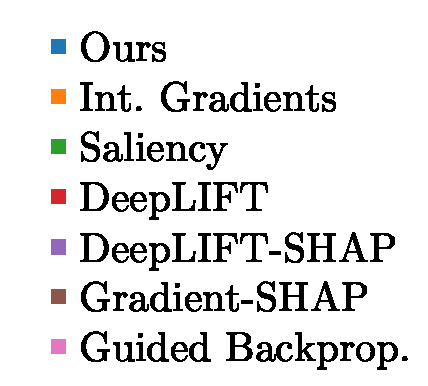
\includegraphics[scale=0.4]{./img/radar-legend.pdf}
    \end{subfigure}
    \caption{Radar plot of the quantitative metrics for the multimodal tasks. The closer to the center, the better.} \label{fig:radar_mm}
\end{figure}

For a qualitative evaluation, we analyze 100 samples from Flickr8k. We observed a consistent behavior as for text and image modality alone. The attribution maps that our method produces tend to be more well separated in terms of score magnitude, allowing to more clearly distinguish what is relevant. Also, as it does not lose in terms of faithfulness, what the scores give high relevance tend to usually be the object of interest in both the text sequence and figure. We provide a sample from the dataset in \Cref{fig:flickr8k_sample}.

\begin{figure}[t!]
    \centering
    \footnotesize
    \begin{subfigure}[b]{0.32\linewidth}
        \centering
        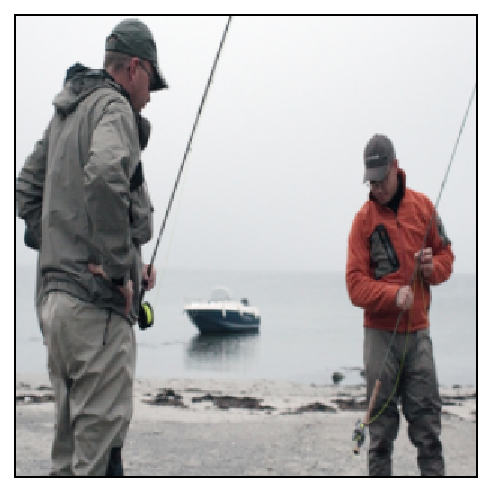
\includegraphics[width=0.8\linewidth]{./img/flickr8k.pdf}
    \end{subfigure}
    \begin{subfigure}[b]{0.32\linewidth}
        \centering
        \textbf{Ours} \\[-0.5em] {\scriptsize\tt\colorbox[RGB]{255, 247, 236}{\textcolor{black}{\vphantom{Tg}Men}} \colorbox[RGB]{127, 0, 0}{\textcolor{white}{\vphantom{Tg}standing}} \colorbox[RGB]{127, 0, 0}{\textcolor{white}{\vphantom{Tg}on}} \colorbox[RGB]{127, 0, 0}{\textcolor{white}{\vphantom{Tg}shore}} \colorbox[RGB]{127, 0, 0}{\textcolor{white}{\vphantom{Tg}with}} \colorbox[RGB]{127, 0, 0}{\textcolor{white}{\vphantom{Tg}fishing}} \colorbox[RGB]{127, 0, 0}{\textcolor{white}{\vphantom{Tg}pole}} \colorbox[RGB]{255, 247, 236}{\textcolor{black}{\vphantom{Tg}and}} \colorbox[RGB]{255, 247, 236}{\textcolor{black}{\vphantom{Tg}boat}} \colorbox[RGB]{255, 247, 236}{\textcolor{black}{\vphantom{Tg}in}} \colorbox[RGB]{252, 140, 89}{\textcolor{black}{\vphantom{Tg}water</s>}}}
        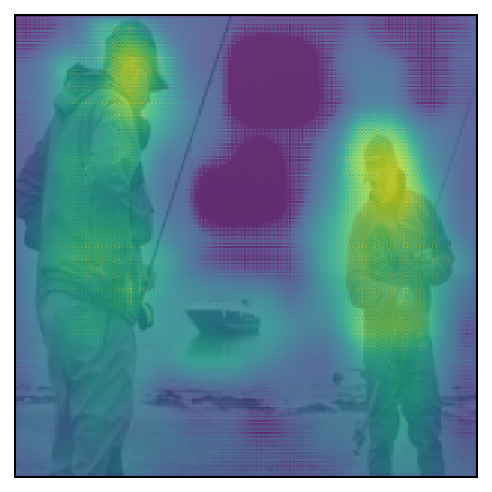
\includegraphics[width=0.8\linewidth]{./img/flickr8k-our.pdf}
    \end{subfigure}
    \begin{subfigure}[b]{0.32\linewidth}
        \centering
        \textbf{Saliency} \\[-0.5em] {\scriptsize\tt\colorbox[RGB]{253, 209, 155}{\textcolor{black}{\vphantom{Tg}Men}} \colorbox[RGB]{249, 130, 84}{\textcolor{black}{\vphantom{Tg}standing}} \colorbox[RGB]{252, 150, 98}{\textcolor{black}{\vphantom{Tg}on}} \colorbox[RGB]{253, 204, 150}{\textcolor{black}{\vphantom{Tg}shore}} \colorbox[RGB]{253, 218, 171}{\textcolor{black}{\vphantom{Tg}with}} \colorbox[RGB]{253, 179, 125}{\textcolor{black}{\vphantom{Tg}fishing}} \colorbox[RGB]{230, 82, 57}{\textcolor{black}{\vphantom{Tg}pole}} \colorbox[RGB]{127, 0, 0}{\textcolor{white}{\vphantom{Tg}and}} \colorbox[RGB]{250, 135, 87}{\textcolor{black}{\vphantom{Tg}boat}} \colorbox[RGB]{225, 70, 48}{\textcolor{black}{\vphantom{Tg}in}} \colorbox[RGB]{251, 138, 88}{\textcolor{black}{\vphantom{Tg}water</s>}}}\\
        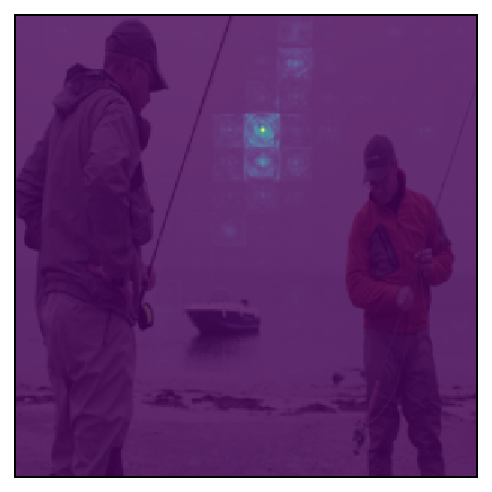
\includegraphics[width=0.8\linewidth]{./img/flickr8k-saliency.pdf}
    \end{subfigure}

    \vspace*{1em}
    
    \begin{subfigure}[b]{0.32\linewidth}
        \centering
        \textbf{Int. Gradients} \\[-0.5em] {\scriptsize\tt\colorbox[RGB]{253, 219, 172}{\textcolor{black}{\vphantom{Tg}Men}} \colorbox[RGB]{254, 223, 180}{\textcolor{black}{\vphantom{Tg}standing}} \colorbox[RGB]{254, 234, 204}{\textcolor{black}{\vphantom{Tg}on}} \colorbox[RGB]{253, 197, 142}{\textcolor{black}{\vphantom{Tg}shore}} \colorbox[RGB]{253, 175, 121}{\textcolor{black}{\vphantom{Tg}with}} \colorbox[RGB]{127, 0, 0}{\textcolor{white}{\vphantom{Tg}fishing}} \colorbox[RGB]{254, 239, 217}{\textcolor{black}{\vphantom{Tg}pole}} \colorbox[RGB]{253, 166, 113}{\textcolor{black}{\vphantom{Tg}and}} \colorbox[RGB]{249, 130, 84}{\textcolor{black}{\vphantom{Tg}boat}} \colorbox[RGB]{255, 247, 236}{\textcolor{black}{\vphantom{Tg}in}} \colorbox[RGB]{253, 166, 113}{\textcolor{black}{\vphantom{Tg}water</s>}}}\\
        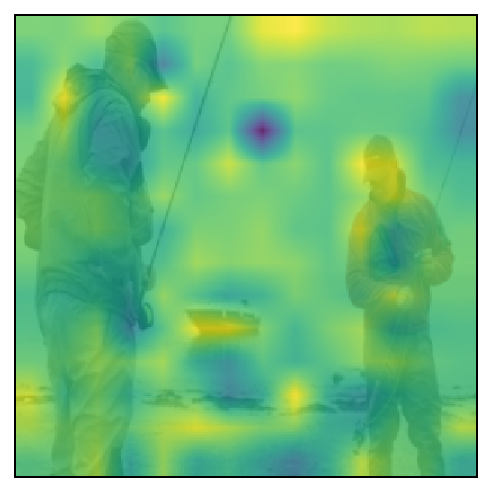
\includegraphics[width=0.8\linewidth]{./img/flickr8k-ig.pdf}
    \end{subfigure}
    \begin{subfigure}[b]{0.32\linewidth}
        \centering
        \textbf{DeepLIFT} \\[-0.5em] {\scriptsize\tt\colorbox[RGB]{233, 87, 61}{\textcolor{black}{\vphantom{Tg}Men}} \colorbox[RGB]{225, 70, 48}{\textcolor{black}{\vphantom{Tg}standing}} \colorbox[RGB]{205, 35, 22}{\textcolor{white}{\vphantom{Tg}on}} \colorbox[RGB]{218, 55, 36}{\textcolor{black}{\vphantom{Tg}shore}} \colorbox[RGB]{245, 120, 80}{\textcolor{black}{\vphantom{Tg}with}} \colorbox[RGB]{252, 162, 109}{\textcolor{black}{\vphantom{Tg}fishing}} \colorbox[RGB]{127, 0, 0}{\textcolor{white}{\vphantom{Tg}pole}} \colorbox[RGB]{223, 67, 45}{\textcolor{black}{\vphantom{Tg}and}} \colorbox[RGB]{255, 247, 236}{\textcolor{black}{\vphantom{Tg}boat}} \colorbox[RGB]{224, 68, 47}{\textcolor{black}{\vphantom{Tg}in}} \colorbox[RGB]{252, 140, 89}{\textcolor{black}{\vphantom{Tg}water</s>}}}\\
        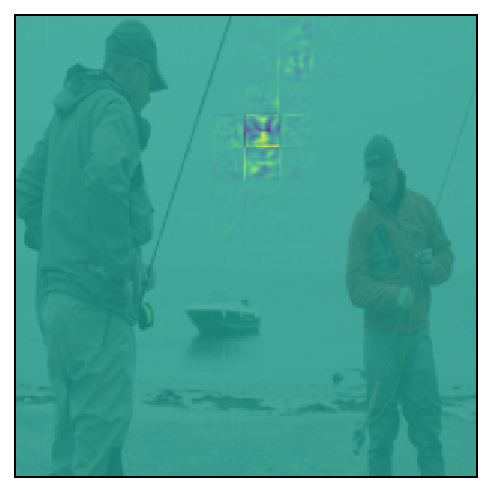
\includegraphics[width=0.8\linewidth]{./img/flickr8k-deeplift.pdf}
    \end{subfigure}
    \begin{subfigure}[b]{0.32\linewidth}
        \centering
        \textbf{DeepLIFT-SHAP} \\[-0.5em] {\scriptsize\tt\colorbox[RGB]{240, 105, 74}{\textcolor{black}{\vphantom{Tg}Men}} \colorbox[RGB]{244, 117, 79}{\textcolor{black}{\vphantom{Tg}standing}} \colorbox[RGB]{185, 8, 5}{\textcolor{white}{\vphantom{Tg}on}} \colorbox[RGB]{223, 65, 44}{\textcolor{black}{\vphantom{Tg}shore}} \colorbox[RGB]{244, 117, 79}{\textcolor{black}{\vphantom{Tg}with}} \colorbox[RGB]{253, 200, 146}{\textcolor{black}{\vphantom{Tg}fishing}} \colorbox[RGB]{127, 0, 0}{\textcolor{white}{\vphantom{Tg}pole}} \colorbox[RGB]{224, 68, 47}{\textcolor{black}{\vphantom{Tg}and}} \colorbox[RGB]{255, 247, 236}{\textcolor{black}{\vphantom{Tg}boat}} \colorbox[RGB]{143, 0, 0}{\textcolor{white}{\vphantom{Tg}in}} \colorbox[RGB]{252, 146, 94}{\textcolor{black}{\vphantom{Tg}water</s>}}}\\
        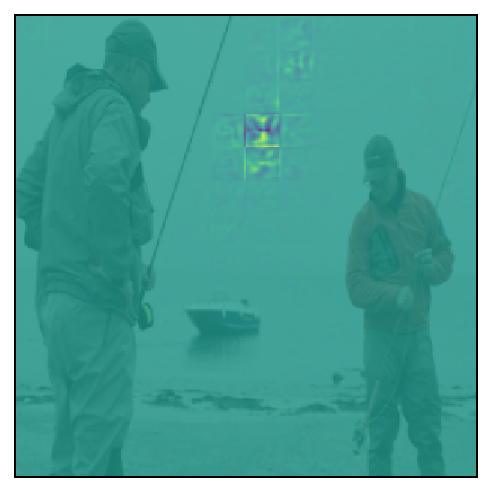
\includegraphics[width=0.8\linewidth]{./img/flickr8k-deepliftshap.pdf}
    \end{subfigure}

    \vspace*{1em}   

    \begin{subfigure}[b]{0.32\linewidth}
        \centering
        \textbf{Gradient-SHAP} \\[-0.5em] {\scriptsize\tt\colorbox[RGB]{252, 163, 110}{\textcolor{black}{\vphantom{Tg}Men}} \colorbox[RGB]{169, 0, 0}{\textcolor{white}{\vphantom{Tg}standing}} \colorbox[RGB]{127, 0, 0}{\textcolor{white}{\vphantom{Tg}on}} \colorbox[RGB]{216, 50, 33}{\textcolor{black}{\vphantom{Tg}shore}} \colorbox[RGB]{253, 194, 139}{\textcolor{black}{\vphantom{Tg}with}} \colorbox[RGB]{253, 184, 129}{\textcolor{black}{\vphantom{Tg}fishing}} \colorbox[RGB]{241, 106, 74}{\textcolor{black}{\vphantom{Tg}pole}} \colorbox[RGB]{254, 226, 188}{\textcolor{black}{\vphantom{Tg}and}} \colorbox[RGB]{252, 150, 98}{\textcolor{black}{\vphantom{Tg}boat}} \colorbox[RGB]{255, 247, 236}{\textcolor{black}{\vphantom{Tg}in}} \colorbox[RGB]{240, 103, 73}{\textcolor{black}{\vphantom{Tg}water</s>}}}\\
        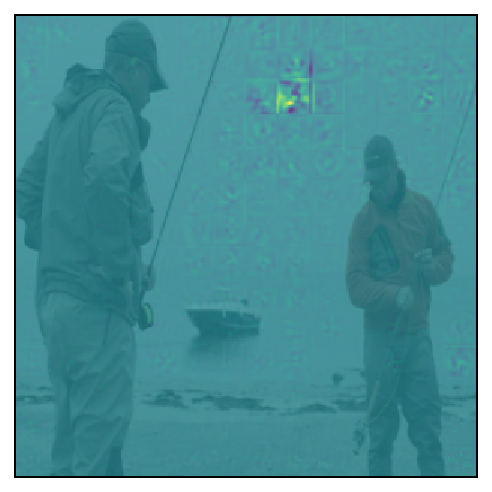
\includegraphics[width=0.8\linewidth]{./img/flickr8k-gradientshap.pdf}
    \end{subfigure}
    \begin{subfigure}[b]{0.32\linewidth}
        \centering
        \textbf{Guided backprop} \\[-0.5em] {\scriptsize\tt\colorbox[RGB]{254, 225, 185}{\textcolor{black}{\vphantom{Tg}Men}} \colorbox[RGB]{176, 0, 0}{\textcolor{white}{\vphantom{Tg}standing}} \colorbox[RGB]{250, 135, 87}{\textcolor{black}{\vphantom{Tg}on}} \colorbox[RGB]{254, 227, 189}{\textcolor{black}{\vphantom{Tg}shore}} \colorbox[RGB]{253, 195, 141}{\textcolor{black}{\vphantom{Tg}with}} \colorbox[RGB]{238, 98, 70}{\textcolor{black}{\vphantom{Tg}fishing}} \colorbox[RGB]{255, 247, 236}{\textcolor{black}{\vphantom{Tg}pole}} \colorbox[RGB]{127, 0, 0}{\textcolor{white}{\vphantom{Tg}and}} \colorbox[RGB]{240, 104, 73}{\textcolor{black}{\vphantom{Tg}boat}} \colorbox[RGB]{140, 0, 0}{\textcolor{white}{\vphantom{Tg}in}} \colorbox[RGB]{224, 68, 47}{\textcolor{black}{\vphantom{Tg}water</s>}}}\\
        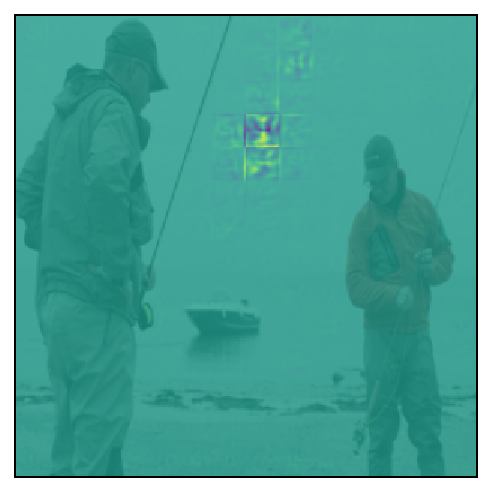
\includegraphics[width=0.8\linewidth]{./img/flickr8k-guidedbackprop.pdf}
    \end{subfigure}
    \caption{Sample from Flickr8k} \label{fig:flickr8k_sample}
\end{figure}

Overall, also in the case of multimodal classification, our method performs consistently by producing attribution maps with relatively low complexity and high sparsity while maintaining reasonable average drop and deletion AUC, highlighting again a good trade-off between visually appealing and faithful attribution maps compared to the other baselines that tend to favor only one side.



\section{Ablation Study}

To empirically experiment with the effectiveness of our design choices, we analyze the impact of the key components of our method. For computational efficiency, we limit ablation study to Tweet Sentiment Extraction and Imagenette to cover both modalities. We aim at testing whether the architectural choices and the training routine are effective. Therefore, we experiment with:
\begin{enumerate*}
    \item removing the last ReLU activation,
    \item removing the last sigmoid activation,
    \item removing the last rescaling step,
    \item removing the binary penalty in the loss,
    \item removing the magnitude penalty in the loss,
    \item removing the penalty in the loss completely,
    \item remove every component we introduce and train the model with only cross-entropy.
\end{enumerate*}

Results on Tweet Sentiment Extraction are presented in \Cref{tab:tweet_ablation} and a sample from the dataset is presented in \Cref{fig:tweet_ablation}. In terms of architecture, we can observe that, by either removing the final ReLU, sigmoid, or rescaling, there is a worsening in sparsity and an improvement in average drop and deletion AUC. This indicates, also as we can observe in \Cref{fig:tweet_ablation}, that the attribution maps becomes more expansive and considers more input tokens as relevant. Also in terms of loss function, we can observe that, after removing each component, results are decreased across all metrics. Finally, if everything is excluded, we can see that the method performs well in terms of average drop and deletion AUC, while it worsens in complexity and sparsity, indicating that the attribution map, without constraints, becomes trivially a non-informative result.


\begin{table}[t!]
    \centering
    \caption{Ablation results on Tweet Sentiment Extraction} \label{tab:tweet_ablation}
    \small
    \def\arraystretch{0.75}
    \makebox[\linewidth][c]{%
    \begin{tabular}{lcccc}
        \toprule
        \textbf{Method} & \textbf{Average drop $\downarrow$} & \textbf{Deletion AUC $\downarrow$} & \textbf{Complexity $\downarrow$} & \textbf{Sparsity $\uparrow$} \\
        \midrule
        Full              & 1.11 \std{1.52} & 1.61 \std{1.57} & 2.71 \std{1.04} & 87.21 \std{72.40} \\
        \midrule
        No ReLU           & 0.38 \std{0.58} & 0.66 \std{0.62} & 2.40 \std{0.68} & 81.95 \std{49.85} \\
        No sigmoid        & 1.28 \std{1.73} & 1.49 \std{1.63} & 3.04 \std{0.82} & 67.04 \std{53.80} \\
        No rescale        & 0.00 \std{0.01} & 0.17 \std{0.13} & 4.25 \std{0.96} & 32.32 \std{17.15} \\
        No binary pen.    & 1.26 \std{1.73} & 1.49 \std{1.69} & 3.16 \std{0.89} & 65.08 \std{53.13} \\
        No magnitude pen. & 1.29 \std{1.73} & 1.42 \std{1.68} & 3.35 \std{1.00} & 64.04 \std{53.90} \\
        No penalty        & 1.27 \std{1.73} & 1.40 \std{1.68} & 3.37 \std{1.02} & 63.76 \std{54.10} \\
        Nothing           & 0.06 \std{0.15} & 0.97 \std{0.77} & 3.19 \std{0.85} & 43.03 \std{26.78} \\
        \bottomrule
    \end{tabular}
    }
\end{table}

\begin{figure}[t!]
    \scriptsize
    \centering
    \makebox[\linewidth][c]{%
    \begin{tabular}{lc}
    \textbf{Full} & {\tt\colorbox[RGB]{127, 0, 0}{\textcolor{white}{\vphantom{Tg}I}} \colorbox[RGB]{127, 0, 0}{\textcolor{white}{\vphantom{Tg}want}} \colorbox[RGB]{255, 247, 236}{\textcolor{black}{\vphantom{Tg}cookies}} \colorbox[RGB]{255, 247, 236}{\textcolor{black}{\vphantom{Tg}for}} \colorbox[RGB]{252, 140, 89}{\textcolor{black}{\vphantom{Tg}breakfast!}} \colorbox[RGB]{255, 247, 236}{\textcolor{black}{\vphantom{Tg}Luckily}} \colorbox[RGB]{253, 195, 141}{\textcolor{black}{\vphantom{Tg}I`m}} \colorbox[RGB]{127, 0, 0}{\textcolor{white}{\vphantom{Tg}an}} \colorbox[RGB]{127, 0, 0}{\textcolor{white}{\vphantom{Tg}adult}} \colorbox[RGB]{255, 247, 236}{\textcolor{black}{\vphantom{Tg}and}} \colorbox[RGB]{127, 0, 0}{\textcolor{white}{\vphantom{Tg}can}} \colorbox[RGB]{127, 0, 0}{\textcolor{white}{\vphantom{Tg}do}} \colorbox[RGB]{231, 83, 58}{\textcolor{black}{\vphantom{Tg}that!</s>}}}\\
    \textbf{No ReLU} & {\tt\colorbox[RGB]{253, 215, 164}{\textcolor{black}{\vphantom{Tg}I}} \colorbox[RGB]{254, 237, 211}{\textcolor{black}{\vphantom{Tg}want}} \colorbox[RGB]{254, 239, 216}{\textcolor{black}{\vphantom{Tg}cookies}} \colorbox[RGB]{255, 247, 236}{\textcolor{black}{\vphantom{Tg}for}} \colorbox[RGB]{253, 184, 129}{\textcolor{black}{\vphantom{Tg}breakfast!}} \colorbox[RGB]{127, 0, 0}{\textcolor{white}{\vphantom{Tg}Luckily}} \colorbox[RGB]{253, 171, 117}{\textcolor{black}{\vphantom{Tg}I`m}} \colorbox[RGB]{253, 200, 146}{\textcolor{black}{\vphantom{Tg}an}} \colorbox[RGB]{253, 221, 177}{\textcolor{black}{\vphantom{Tg}adult}} \colorbox[RGB]{253, 176, 122}{\textcolor{black}{\vphantom{Tg}and}} \colorbox[RGB]{253, 192, 137}{\textcolor{black}{\vphantom{Tg}can}} \colorbox[RGB]{253, 217, 168}{\textcolor{black}{\vphantom{Tg}do}} \colorbox[RGB]{253, 197, 142}{\textcolor{black}{\vphantom{Tg}that!</s>}}}\\
    \textbf{No sigmoid} & {\tt\colorbox[RGB]{127, 0, 0}{\textcolor{white}{\vphantom{Tg}I}} \colorbox[RGB]{255, 247, 236}{\textcolor{black}{\vphantom{Tg}want}} \colorbox[RGB]{255, 247, 236}{\textcolor{black}{\vphantom{Tg}cookies}} \colorbox[RGB]{255, 247, 236}{\textcolor{black}{\vphantom{Tg}for}} \colorbox[RGB]{255, 247, 236}{\textcolor{black}{\vphantom{Tg}breakfast!}} \colorbox[RGB]{127, 0, 0}{\textcolor{white}{\vphantom{Tg}Luckily}} \colorbox[RGB]{231, 83, 58}{\textcolor{black}{\vphantom{Tg}I`m}} \colorbox[RGB]{127, 0, 0}{\textcolor{white}{\vphantom{Tg}an}} \colorbox[RGB]{127, 0, 0}{\textcolor{white}{\vphantom{Tg}adult}} \colorbox[RGB]{255, 247, 236}{\textcolor{black}{\vphantom{Tg}and}} \colorbox[RGB]{127, 0, 0}{\textcolor{white}{\vphantom{Tg}can}} \colorbox[RGB]{127, 0, 0}{\textcolor{white}{\vphantom{Tg}do}} \colorbox[RGB]{231, 83, 58}{\textcolor{black}{\vphantom{Tg}that!</s>}}}\\
    \textbf{No rescale} & {\tt\colorbox[RGB]{140, 0, 0}{\textcolor{white}{\vphantom{Tg}I}} \colorbox[RGB]{147, 0, 0}{\textcolor{white}{\vphantom{Tg}want}} \colorbox[RGB]{140, 0, 0}{\textcolor{white}{\vphantom{Tg}cookies}} \colorbox[RGB]{151, 0, 0}{\textcolor{white}{\vphantom{Tg}for}} \colorbox[RGB]{151, 0, 0}{\textcolor{white}{\vphantom{Tg}breakfast!}} \colorbox[RGB]{156, 0, 0}{\textcolor{white}{\vphantom{Tg}Luckily}} \colorbox[RGB]{148, 0, 0}{\textcolor{white}{\vphantom{Tg}I`m}} \colorbox[RGB]{148, 0, 0}{\textcolor{white}{\vphantom{Tg}an}} \colorbox[RGB]{134, 0, 0}{\textcolor{white}{\vphantom{Tg}adult}} \colorbox[RGB]{127, 0, 0}{\textcolor{white}{\vphantom{Tg}and}} \colorbox[RGB]{138, 0, 0}{\textcolor{white}{\vphantom{Tg}can}} \colorbox[RGB]{137, 0, 0}{\textcolor{white}{\vphantom{Tg}do}} \colorbox[RGB]{137, 0, 0}{\textcolor{white}{\vphantom{Tg}that!</s>}}}\\
    \textbf{No binary pen.} & {\tt\colorbox[RGB]{127, 0, 0}{\textcolor{white}{\vphantom{Tg}I}} \colorbox[RGB]{255, 247, 236}{\textcolor{black}{\vphantom{Tg}want}} \colorbox[RGB]{255, 247, 236}{\textcolor{black}{\vphantom{Tg}cookies}} \colorbox[RGB]{255, 247, 236}{\textcolor{black}{\vphantom{Tg}for}} \colorbox[RGB]{255, 247, 236}{\textcolor{black}{\vphantom{Tg}breakfast!}} \colorbox[RGB]{127, 0, 0}{\textcolor{white}{\vphantom{Tg}Luckily}} \colorbox[RGB]{231, 83, 58}{\textcolor{black}{\vphantom{Tg}I`m}} \colorbox[RGB]{127, 0, 0}{\textcolor{white}{\vphantom{Tg}an}} \colorbox[RGB]{127, 0, 0}{\textcolor{white}{\vphantom{Tg}adult}} \colorbox[RGB]{255, 247, 236}{\textcolor{black}{\vphantom{Tg}and}} \colorbox[RGB]{127, 0, 0}{\textcolor{white}{\vphantom{Tg}can}} \colorbox[RGB]{127, 0, 0}{\textcolor{white}{\vphantom{Tg}do}} \colorbox[RGB]{231, 83, 58}{\textcolor{black}{\vphantom{Tg}that!</s>}}}\\
    \textbf{No magnitude pen.} & {\tt\colorbox[RGB]{127, 0, 0}{\textcolor{white}{\vphantom{Tg}I}} \colorbox[RGB]{255, 247, 236}{\textcolor{black}{\vphantom{Tg}want}} \colorbox[RGB]{255, 247, 236}{\textcolor{black}{\vphantom{Tg}cookies}} \colorbox[RGB]{255, 247, 236}{\textcolor{black}{\vphantom{Tg}for}} \colorbox[RGB]{255, 247, 236}{\textcolor{black}{\vphantom{Tg}breakfast!}} \colorbox[RGB]{127, 0, 0}{\textcolor{white}{\vphantom{Tg}Luckily}} \colorbox[RGB]{231, 83, 58}{\textcolor{black}{\vphantom{Tg}I`m}} \colorbox[RGB]{127, 0, 0}{\textcolor{white}{\vphantom{Tg}an}} \colorbox[RGB]{127, 0, 0}{\textcolor{white}{\vphantom{Tg}adult}} \colorbox[RGB]{255, 247, 236}{\textcolor{black}{\vphantom{Tg}and}} \colorbox[RGB]{127, 0, 0}{\textcolor{white}{\vphantom{Tg}can}} \colorbox[RGB]{127, 0, 0}{\textcolor{white}{\vphantom{Tg}do}} \colorbox[RGB]{231, 83, 58}{\textcolor{black}{\vphantom{Tg}that!</s>}}}\\
    \textbf{No penalty} & {\tt\colorbox[RGB]{127, 0, 0}{\textcolor{white}{\vphantom{Tg}I}} \colorbox[RGB]{255, 247, 236}{\textcolor{black}{\vphantom{Tg}want}} \colorbox[RGB]{255, 247, 236}{\textcolor{black}{\vphantom{Tg}cookies}} \colorbox[RGB]{255, 247, 236}{\textcolor{black}{\vphantom{Tg}for}} \colorbox[RGB]{255, 247, 236}{\textcolor{black}{\vphantom{Tg}breakfast!}} \colorbox[RGB]{127, 0, 0}{\textcolor{white}{\vphantom{Tg}Luckily}} \colorbox[RGB]{231, 83, 58}{\textcolor{black}{\vphantom{Tg}I`m}} \colorbox[RGB]{127, 0, 0}{\textcolor{white}{\vphantom{Tg}an}} \colorbox[RGB]{127, 0, 0}{\textcolor{white}{\vphantom{Tg}adult}} \colorbox[RGB]{255, 247, 236}{\textcolor{black}{\vphantom{Tg}and}} \colorbox[RGB]{127, 0, 0}{\textcolor{white}{\vphantom{Tg}can}} \colorbox[RGB]{127, 0, 0}{\textcolor{white}{\vphantom{Tg}do}} \colorbox[RGB]{231, 83, 58}{\textcolor{black}{\vphantom{Tg}that!</s>}}}\\
    \textbf{Nothing} & {\tt\colorbox[RGB]{224, 68, 47}{\textcolor{black}{\vphantom{Tg}I}} \colorbox[RGB]{178, 0, 0}{\textcolor{white}{\vphantom{Tg}want}} \colorbox[RGB]{180, 2, 1}{\textcolor{white}{\vphantom{Tg}cookies}} \colorbox[RGB]{189, 14, 9}{\textcolor{white}{\vphantom{Tg}for}} \colorbox[RGB]{219, 57, 38}{\textcolor{black}{\vphantom{Tg}breakfast!}} \colorbox[RGB]{252, 142, 90}{\textcolor{black}{\vphantom{Tg}Luckily}} \colorbox[RGB]{227, 75, 52}{\textcolor{black}{\vphantom{Tg}I`m}} \colorbox[RGB]{226, 73, 51}{\textcolor{black}{\vphantom{Tg}an}} \colorbox[RGB]{211, 42, 27}{\textcolor{white}{\vphantom{Tg}adult}} \colorbox[RGB]{236, 95, 67}{\textcolor{black}{\vphantom{Tg}and}} \colorbox[RGB]{193, 18, 12}{\textcolor{white}{\vphantom{Tg}can}} \colorbox[RGB]{224, 68, 47}{\textcolor{black}{\vphantom{Tg}do}} \colorbox[RGB]{210, 41, 26}{\textcolor{white}{\vphantom{Tg}that!</s>}}}\\
    \end{tabular}
    }
    \caption{Ablation results on a sample from Tweet Sentiment Extraction} \label{fig:tweet_ablation}
\end{figure}


Ablation results on Imagenette are presented in \Cref{tab:imagenette_ablation} and a sample for qualitative analysis is shown in \Cref{fig:imagenette_ablation}. As for text, in all cases, but the scenario where rescaling is removed, performance on complexity and sparsity tend to worsen. In the case of rescaling, the behavior is opposite as average drop and deletion AUC worsen but complexity and sparsity improve. However, qualitatively we can see that the best result is obtained with every component as they allow to obtain a clearer distinction between what is relevant in the input.

\begin{table}[t!]
    \centering
    \caption{Ablation results on Imagenette} \label{tab:imagenette_ablation}
    \small
    \def\arraystretch{0.75}
    \makebox[\linewidth][c]{%
    \begin{tabular}{lcccc}
        \toprule
        \textbf{Method} & \textbf{Average drop $\downarrow$} & \textbf{Deletion AUC $\downarrow$} & \textbf{Complexity $\downarrow$} & \textbf{Sparsity $\uparrow$} \\
        \midrule
        Full               & 0.02 \std{0.07} & 0.27 \std{0.12} & 60.43  \std{19.45} & 7.02  \std{2.92} \\
        \midrule
        No ReLU            & 0.02 \std{0.06} & 0.30 \std{0.15} & 64.89  \std{18.82} & 4.74  \std{1.70} \\
        No sigmoid         & 0.02 \std{0.05} & 0.29 \std{0.12} & 60.31  \std{19.83} & 6.14  \std{2.82} \\
        No rescale         & 0.34 \std{0.26} & 0.45 \std{0.18} & 43.44  \std{46.93} & 22.03 \std{24.26} \\
        No binary pen.     & 0.02 \std{0.06} & 0.37 \std{0.09} & 48.68  \std{13.85} & 6.81  \std{3.45} \\
        No magnitude pen.  & 0.01 \std{0.03} & 0.04 \std{0.03} & 159.79 \std{25.34} & 1.92  \std{0.88} \\
        No penalty penalty & 0.01 \std{0.04} & 0.08 \std{0.07} & 149.04 \std{24.68} & 1.98  \std{0.78} \\
        Nothing            & 0.01 \std{0.02} & 0.06 \std{0.07} & 161.76 \std{30.60} & 1.56  \std{0.59} \\
        \bottomrule
    \end{tabular}
    }
\end{table}

\begin{figure}[t!]
    \centering
    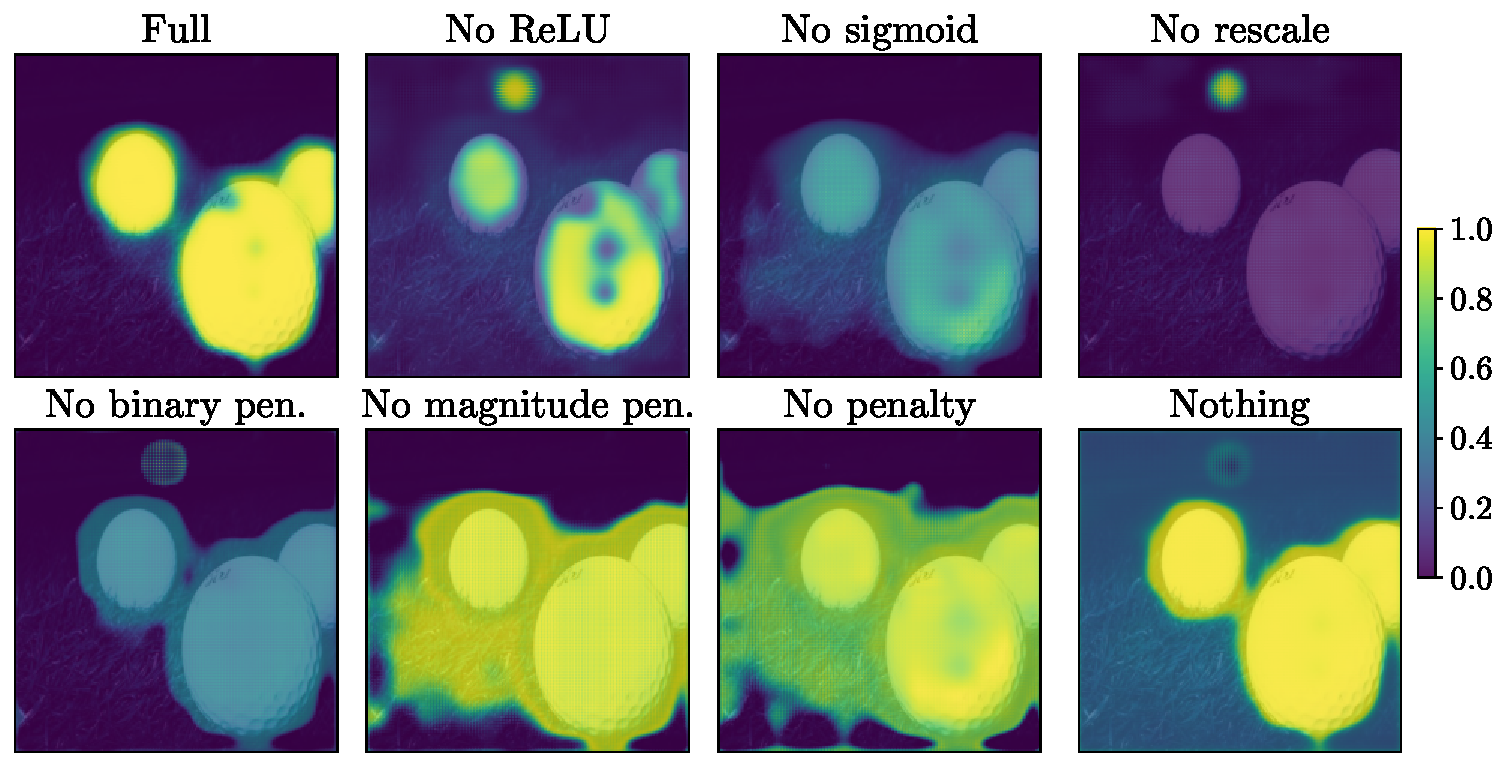
\includegraphics[width=0.9\linewidth]{./img/imagenette-ablation.pdf}
    \caption{Ablation results on a sample from Imagenette} \label{fig:imagenette_ablation}
\end{figure}